\chapter{Verwendete Myonen Simulationssoftware}

Dieser Abschnitt führt die Myonen Simulationssoftwares,
EcoMug und PROPOSAL ein.

\section{Myonen Erzeugung mit EcoMug}

% EcoMug ist eine reine C++11-Header-Bibliothek 
% zur Erzeugung von Myonen aus kosmischer Strahlung 
% (CR), die auf einer Parametrisierung experimenteller 
% Daten basiert. Im Gegensatz zu anderen Werkzeugen 
% bietet EcoMug die Möglichkeit, aus verschiedenen Oberflächen 
% (Ebene, Zylinder und Halbkugel) zu erzeugen, wobei die 
% korrekte  der erzeugten Spuren 
% erhalten bleibt. EcoMug ermöglicht auch die Erzeugung von 
% CR-Myonen nach benutzerdefinierten Parametrisierungen ihres 
% differentiellen Flusses.

EcoMug\footnote{\url{https://github.com/dr4kan/EcoMug}} ist ein C++-Programm 
zur Generierung einzelner Myonen \cite{EcoMug} anhand einer
Parametrisierung des differentiellen Myonenflusses. 

Es lässt sich neben dem standardmäßig implementierten Myonenfluss
auch ein eigener definieren.
Außerdem bietet EcoMug die Möglichkeit, Myonen aus verschiedenen Oberflächen (Ebene, Zylinder und Halbkugel) mit physikalisch korrekter
Winkel- und Impulsverteilung zu erzeugen. 
Zu guter Letzt ist EcoMug mit besonderem Merkmal auf Schnelligkeit entwickelt worden.



\section{Lepton Propagation mit PROPOSAL}

PROPOSAL\footnote{\url{https://github.com/tudo-astroparticlephysics/PROPOSAL}} ist ein in C++ geschriebenes Simulationsprogramm und steht für 
\textbf{Pr}opagator with \textbf{O}ptimal \textbf{P}recision 
and \textbf{O}ptimized \textbf{S}peed for \textbf{A}ll \textbf{L}eptons. 
\cite{proposal, proposal2, proposal3}
%  nahe dem geografischen Südpol in der Antarktis.
Über den Monte-Carlo-Algorithmus lassen sich Leptonen wie
Elektronen, Myonen und Taus durch verschiedene Medien propagieren. 
% Propagieren bedeutet, dass die Wechselwirkungen des Teilchens mit
% der Materie durch das es fliegt simuliert wird.
PROPOSAL kann den Energieverlust, Ablenkung sowie Zerfall der Teilchen simulieren.
% Bei Zusammenstößen mit Materie verliert es Energie und ändert seine Richtung.

PROPOSAL wird hauptsächlich an der TU Dortmund weiterentwickelt 
sowie als OpenSource Projekt auf GitHub. 
Es ist unter anderem ein Bestandteil der Simulationskette des Neutrino-Detektors IceCube \cite{icecube}.
Im Vergleich dazu sei auch das Simulationsprogramm GEANT4 erwähnt, welches speziell
für die Simulation von Teilchen innerhalb eines Detektors konzipiert ist.
PROPOSAL ist dahingehend optimiert, über längere Strecken ($> \SI[]{1}[]{km}$) Teilchen 
zu propagieren, daher ist es auch für die Anwendung in der Myographie
gut geeignet.

\subsection{Funktionsweise von PROPOSAL}
\label{sec:pp-theorie}

In PROPOSAL sind für die Propagation von Myonen die Wirkungsquerschnitte für 
Ionisation, Bremsstrahlung, Paarproduktion und Photonukleare Wechselwirkung 
implementiert. Außerdem wird der Zerfall anhand der Lebensdauer simuliert. \cite{proposal}
In Abb. \ref{fig:energieverlust_pp} ist der mittlere Energieverlust
der verschiedenen Wechselwirkungen dargestellt.

Die meisten\footnote{Nicht stochastisch bspw.: 
die Dichtekorrektur bei der Ionisation. Sie ist ein rein kontinuierlicher Prozess} 
physikalische Wechselwirkungen sind stochastisch, das heißt
Teilchen verlieren in diskreten Interaktionen Energie bzw. werden abgelenkt.
Die Anzahl an Bremsstrahlungswechselwirkungen divergieren allerdings für 
immer kleinere Energien gegen unendlich, was bedeuten würde, dass unendlich 
viele Interaktionen berechnet werden müssten. 
Aufgrund dieses Problems und um die Präzision zugunsten der Laufzeit steuern
zu können, gibt es einen frei wählbaren Energieschnitt (Energy-Cut).

\begin{figure}[]
    \centering
    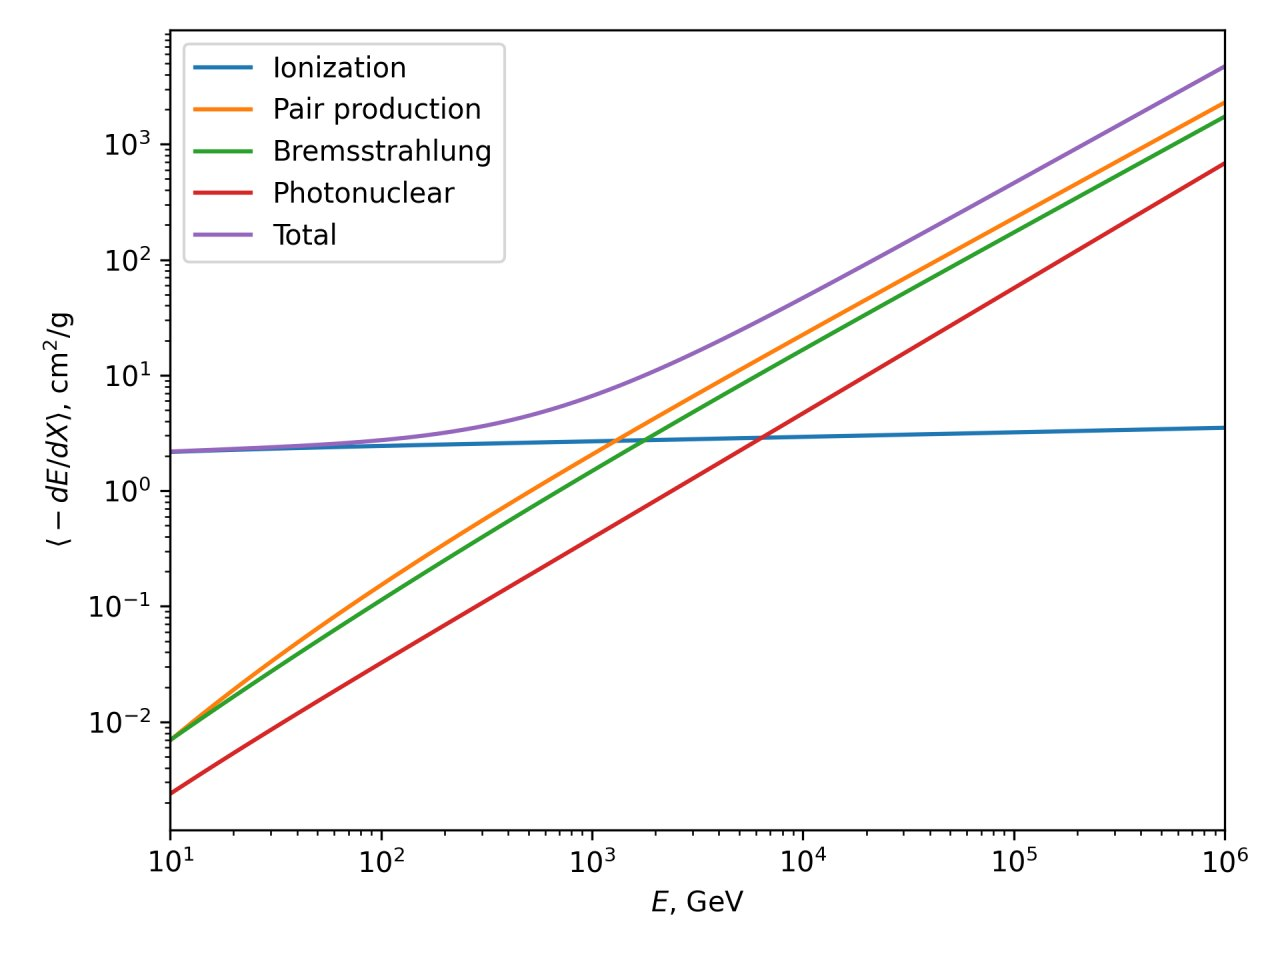
\includegraphics[width=0.55\textwidth]{wechselwirkungen PP.jpg}
    \caption{Der mittleren Energieverlust von Myonen in Standardgestein. Mit PROPOSAL simuliert.}
    \label{fig:energieverlust_pp}
\end{figure}

Der Energy-Cut ist als absoluter $E_\mathrm{cut}$ bzw. relativer $v_\mathrm{cut}$ konfigurierbar.
Unterhalb des Energieschnitts werden die Interaktionen statt stochastisch zufällig gezogen zu werden,
kontinuierlich berechnet.
Das bedeutet, dass ein durchschnittliches $\frac{\mathrm{d}E}{\mathrm{d}x}$
für die kontinuierlichen Energieverluste berechnet wird. 
Dadurch werden die sonst unendlichen Interaktionen der Bremsstrahlung endlich und so simulierbar.
%  \marktodo{warum ist die kont rand wichtig?} 
Es lässt sich optional die sog. kontinuierliche Randomisierung
aktivieren, welche die kontinuierlichen Berechnung über eine Gauß-Verteilung stochastisch verschmiert.
% Die Vielfachstreuung lässt sich optional aktivieren, wobei 3 Parametrisierungen mit 
% unterschiedlichen Approximationen implementiert sind. 
% Davon ist Molière die genauste Implementierung, dann kommt HighlandIntegral als Gaußsche Näherung
% der Molière Parametrisierung. Danach kommt Highland, welches HighlandIntegral ist mit der Annahme, dass 
% die Teilchenenergie während eines Propagationschritts konstant bleibt. 

PROPOSAL wird die Energie, Position, Richtung und Art des zu propagierenden Teilchens 
sowie Sektoren für die Propagation übergeben.
Diese Sektoren werden über eine Liste an implementierten Medien 
und selbst konfigurierbaren Dichte-Verteilungen definiert.
Pro Sektor lässt sich ein individueller Energy-Cut setzen.
Es sind verschiedene Medien wie z. B. Standardgestein oder Wasser implementiert. 
Zudem kann bestimmt werden, wann die Propagation gestoppt werden soll: 
Bis zu einer Energie, nach einer bestimmten Strecke oder 
nach Verlassen eines Sektors.
Zudem muss ein $E_\mathrm{cut}$ bzw. $v_\mathrm{cut}$ gesetzt werden. 
Als Ausgabe übergibt PROPOSAL dem Nutzer ein Objekt \textit{track}, welches 
Informationen über die Propagation des Teilchens innehält.
Es sind unteranderem Endposition, Endenergie und propagierte Strecke abrufbar.  

%  \marktodo{größenordung für vcut und laufzeiten angeben.} 

Genauere Informationen über die Funktionsweise von PROPOSAL lassen sich
aus den Veröffentlichungen \cite{proposal}, \cite{proposal2} und \cite{proposal3} nachlesen.
    

% PROPOSAL hat zwei verschiedene Arten von Tabellen. Einmal die Tabellen für Wirkungsquerschnitte. 
% Da gibt es die Tabellen die dNdx interpolieren. Diese Tabellen sind zweidimensional (in E und v), 
% und das sind deshalb die Tabellen die lange zum bauen brauchen.

% Die anderen Tabellen sind die Tabellen für die “PropagationUtilities”, dessen Stützstellen 
% mit dieser Einstellung verändert werden. Diese werden genutzt, um zum Beispiel die 
% Integralgleichungen zu lösen. Diese Tabellen sind jedoch alle eindimensonal, 
% außerdem basieren sie auf den Interpolationstabllen für die Wirkungsquerschnitte. 
% Deshalb sind die relativ schnell zu bauen.